\chapter*{Wstęp}
\addcontentsline{toc}{chapter}{Wstęp}
\chapter{Wprowadzenie do problematyki}
\chapter{Technologie i narzędzia wykorzystywane w pracy}
\section{Xamarin.Android}
\section{Xamarin.iOS}
\section{ASP.NET Core}
\section{Entity Framework Core}
\section{Dapper}
\section{MVVMCross}
\section{AutoFac}
\section{Team Foundation Server}
\section{HockeyApp}
\section{Microsoft Azure}
\chapter{Założenia projektowe}
\section{Przedmiot pracy}
Przedmiotem pracy jest utworzenie aplikacji mobilnej na platformy Android oraz iOS, umożliwiającej rezerwację i zakup biletów kinowych w ramach sieci kin, wraz z towarzyszącą aplikacją serwerową. Aplikacja kliencka będzie utworzona w oparciu o platformę Xamarin, natomiast aplikacja serwerowa w oparciu o framework ASP.NET Core
\section{Wymagania funkcjonalne}
System powinien spełniać następujące wymagania funkcjonalne. Przy definiowaniu wymagań przyjęto następujących aktorów - Klient, Pracownik kina, Administrator systemu, System
\begin{enumerate}
\item Klient ma możliwość stworzenia konta użytkownika na podstawie adresu e-mail, w celu zachowania preferencji użytkownika pomiędzy urządzeniami.
\item Klient ma możliwość stworzenia konta użytkownika z wykorzystaniem konta w jednym ze wspieranych portali społecznościowych (Facebook, Twitter, Google), w celu przyspieszenia procesu tworzenia konta.
\item Klient ma możliwość modyfikacji informacji o koncie użytkownika.
\item Klient ma możliwość zresetowania hasła do konta użytkownika, w celu odzyskania dostępu do konta. 
\item Klient ma możliwość wyboru domyślnego kina, w celu łatwiejszego dostępu do aktualnego repertuaru.
\item Klient ma możliwość przeglądania aktualnego repertuaru w danym kinie.
\item Klient ma możliwość przeglądania podstawowych informacji o filmie z repertuaru. 
\item Klient ma możliwość złożenia rezerwacji biletu(ów) na wybrany seans w wybranym kinie.
\item Klient ma możliwość modyfikacji wybranej rezerwacji do 30 minut przed planowanym początkiem seansu.
\item System anuluje wszystkie niepotwierdzone rezerwacje 30 minut przed planowanym początkiem seansu. 
\item Klient ma możliwość zakupu biletu(ów) na wybrany seans w wybranym kinie.
\item Klient ma możliwość dokonania zapłaty za zakupione bilety za pośrednictwem zewnętrznego systemu płatności elektronicznych.
\item Klient ma możliwość zwrotu zakupionych biletów do 3 godzin przed planowanym seansem.
\item Klient ma możliwość wyboru miejsc na podstawie widoku sali kinowej.
\item Klient ma możliwość wyboru rodzaju biletu przy wyborze miejsc.
\item Klient ma możliwość przeglądania historii rezerwacji oraz zakupionych biletów.
\item Klient ma możliwość dokonania zakupu biletu(ów) bez potrzeby zakładania konta.
\item Klient ma możliwość dokonania rezerwacji biletu(ów) bez potrzeby zakładania konta. 
\item Klient ma możliwość okazania biletu w formacie kodu QR.
\item Klient ma możliwość okazania biletu pomimo braku połączenia z siecią Internet.\newline
\item Pracownik kina ma możliwość modyfikacji podstawowych danych o kinie.
\item Pracownik kina ma możliwość modyfikacji informacji o salach dostępnych w kinie.
\item Pracownik kina ma możliwość modyfikacji repertuaru kina.
\item Pracownik kina ma możliwość potwierdzenia rezerwacji klienta.
\item Pracownik kina ma możliwość anulowania rezerwacji klienta.
\item Pracownik kina ma możliwość dokonania sprzedaży biletów klientom w kasie biletowej.
\item Administrator systemu ma możliwość dodawania, modyfikowania i usuwania informacji o kinach należących do sieci kin.
\item Administrator systemu ma możliwość tworzenia oraz modyfikacji kont użytkowników oraz przydzielania im ról.
\end{enumerate}
Powyższa lista jest pełnym zbiorem wymagań, które powinny się znaleźć w ostatecznej wersji systemu. Prototyp systemu, będący celem pracy, będzie miał zaimplementowane wszystkie funkcjonalności dotyczące roli Klienta tj. wymagania od pierwszego do dwudziestego.
\section{Wymagania niefunkcjonalne}
Zbiór tych wymagań definiuje, jakie wymagania na system mają zostać spełnione, oprócz wymagań funkcjonalnych. Wymagania te głównie dotyczą wydajności, bezpieczeństwa i tym podobnych aspektów.
\begin{enumerate}
\item System powinien być dostępny bez przerwy. (Dostępność na poziomie 99,9\%)
\item System jest w stanie obsługiwać wiele jednocześnie podłączonych urządzeń.
\item Do poprawnego korzystania ze wszystkich funkcji oferowanych przez aplikację, wymagane jest stałe połączenie internetowe.
\item W celu zapewnienia odpowiedniego poziomu bezpieczeństwa, połączenie między serwerem i klientem ma być szyfrowane.
\item System ma wspierać również mechanizm sesji, jako dodatkowy mechanizm zabezpieczający połączenie.
\item Aplikacja kliencka powinna być dostępna na systemach Android (w wersji 4.4 i wyższej) oraz iOS (w wersji 8.0 i wyższej).
\item Aplikacja kliencka powinna zostać uruchomiona na urządzeniu mobilnym niezależnie od stanu połączenia internetowego.
\item Aplikacja serwerowa powinna móc być uruchomiona na serwerach z systemami rodziny Windows Server (wersja 2012 R2 i wyżej) oraz Linux

\end{enumerate}
\section{Opis podstawowej architektury systemu}
\subsection*{Architektura logiczna}
System będzie składał się z trzech aplikacji. 

\par Pierwszą z nich jest aplikacja serwerowa, realizowana w architekturze trójwarstwowej (podział na warstwę prezentacji, logiki biznesowej oraz dostępu do danych). Dzięki takiemu podziałowi, w którym wyższa warstwa nie wie o logice zawartej w niższej warstwie (\textit{black box}) zapewniamy m.in. dużą skalowalność rozwiązania (każdą warstwę możemy skalować według potrzeb) oraz ułatwione testowanie rozwiązania poprzez brak skomplikowanych zależności pomiędzy warstwami.

\par Operacje na bazie danych aplikacji będą wykonywane w warstwie dostępu do danych z częściowym wykorzystaniem podejścia CQRS (\textit{Command Query Responsibility Segregation}), które zapewni jeszcze lepszą skalowalność rozwiązania poprzez, przede wszystkim oddzielenie operacji zapisu danych od ich odczytu. Więcej szczegółów na temat podejścia CQRS oraz jego implementacji znajduje się w podrozdziale~\ref{sec:cqrs}

\par Pozostałą część systemu stanowią aplikacje mobilne działająca pod kontrolą systemu Android oraz iOS. Aplikacje te będą implementowane z wykorzystaniem platformy Xamarin. Dzięki temu możemy mówić o aplikacji wieloplatformowej, ponieważ większość kodu aplikacji (głównie chodzi tutaj o logikę zawartą w aplikacji) jest współdzielona. Aby umożliwić współdzielenie kodu, będzie zastosowany wzorzec architektoniczny Model-View-ViewModel. Dzięki temu wzorcowi dokonujemy separacji aplikacji na warstwy: widoku (View), logiki interfejsu (ViewModel) oraz modelu danych. Logika interfejsu oraz modelu danych są współdzielone, natomiast osobne widoki odpowiadają specyfice poszczególnych systemów. Wyseparowane warstwy sprawiają, że kod aplikacji jest o wiele bardziej testowalny oraz łatwiejszy w utrzymaniu. Do przechowywania danych lokalnych aplikacji posłuży baza danych SQLite.

\subsection*{Architektura fizyczna}
Aplikacja serwerowa zbudowana będzie w oparciu o framework ASP.NET Core. Będzie mieć ona możliwość pracowania na serwerach z systemami rodziny Windows Server oraz Linux. Wykorzystywany serwer WWW to, w zależności od wybranego systemu, IIS (\textit{Internet Information Services}) oraz Apache.

\par Aplikacja serwerowa będzie komunikować się z serwerem bazodanowym Microsoft SQL Server znajdującym się na osobnym serwerze (działającym pod kontrolą dystrybucji systemu Windows Server lub Linux), z wykorzystaniem protokołu TLS/SSL w celu zapewnienia odpowiedniego poziomu bezpieczeństwa.

\par W ramach realizowanego prototypu, serwery aplikacji oraz bazy danych będą hostowane na platformie obliczeniowej Microsoft Azure. 

\par Aplikacje klienckie działające na urządzeniach z systemami Android oraz iOS, będą komunikowały się z serwerem aplikacji, wykorzystując udostępnione przez aplikację \textit{RESTful API}. Formatem przesyłanych danych jest \textit{JSON}. Komunikacja odbywa się za pośrednictwem protokołu HTTPS (ruch jest szyfrowany).
\begin{figure}[h]
\centering
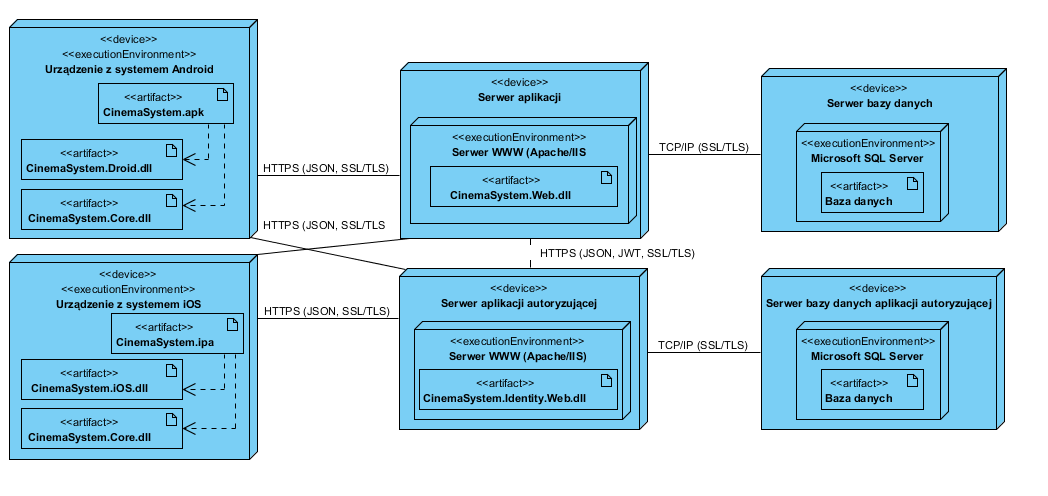
\includegraphics[width=1\textwidth]{img1}
\caption{Architektura fizyczna systemu}
\end{figure}
\chapter{Projekt aplikacji}
\section{Przypadki użycia}
\section{Interfejs}
\section{Diagram klas}
\addtocontents{toc}{\protect\newpage}
\chapter{Implementacja}
\section{DevOps}
\section{Autoryzacja użytkowników aplikacji}
\section{Synchronizacja danych offline-online}
\section{Bezpieczeństwo aplikacji}
\section{Implementacja wzorca CQRS}
\label{sec:cqrs}
\section{Testy interfejsu aplikacji}
\chapter{Podsumowanie}
\bibliographystyle{plain}
\bibliography{./bib/bib} 
\chapter*{Załączniki}
\addcontentsline{toc}{chapter}{Załączniki}
\section*{Spis tabel}
\addcontentsline{toc}{section}{Spis tabel}
\listoftables
\section*{Spis rysunków}
\addcontentsline{toc}{section}{Spis rysunków}
\listoffigures
\lstlistoflistings
\addcontentsline{toc}{section}{Spis listingów}
\section*{Instrukcja kompilacji i testowego uruchomienia aplikacji}
\addcontentsline{toc}{section}{Instrukcja kompilacji i testowego uruchomienia aplikacji}